%%% ======= Beamer ======
\documentclass[usenames,dvipsnames,t]{beamer}
% \documentclass[usenames,dvipsnames, handout]{beamer}
\beamertemplatenavigationsymbolsempty % remove toolbar at the bottom of slides
\usepackage{appendixnumberbeamer} % for appendix
\usetheme{Madrid}
\usecolortheme{default}
\useinnertheme{circles}
\newcommand{\mtov}{M_{\text{TOV}}}

\usepackage{fontawesome}

% Define commands for social media icons with links
\newcommand{\twitter}{\href{https://twitter.com/ThibeauWouters}{\textcolor{black}{\faTwitter}}}
\newcommand{\linkedin}{\href{https://www.linkedin.com/in/ThibeauWouters}{\textcolor{black}{\faLinkedin}}}
\newcommand{\github}{\href{https://github.com/ThibeauWouters}{\textcolor{black}{\faGithub}}}

\setbeamercolor{author in head/foot}{bg=blue!10, fg=blue}
\setbeamercolor{title in head/foot}{bg=blue!10, fg=blue}
\setbeamercolor{date in head/foot}{bg=blue!10, fg=blue}

\makeatletter
\setbeamertemplate{footline}{
  \leavevmode%
  \hbox{%
  \begin{beamercolorbox}[wd=.333333\paperwidth,ht=2.25ex,dp=1ex,center]{author in head/foot}%
    \usebeamerfont{author in head/foot}\insertshortauthor\expandafter\ifblank\expandafter{\beamer@shortinstitute}{}{~~(\insertshortinstitute)}
  \end{beamercolorbox}%
  \begin{beamercolorbox}[wd=.333333\paperwidth,ht=2.25ex,dp=1ex,center]{title in head/foot}%
    \usebeamerfont{title in head/foot}\insertshorttitle
  \end{beamercolorbox}%
  \begin{beamercolorbox}[wd=.333333\paperwidth,ht=2.25ex,dp=1ex,right]{date in head/foot}%
    \usebeamerfont{date in head/foot}\insertshortdate{}\hspace*{2em}
    \insertframenumber{}%
%     / \inserttotalframenumber
    \hspace*{2ex} 
  \end{beamercolorbox}}%
  \vskip0pt%
}
\makeatother

\colorlet{beamer@blendedblue}{blue!70} % change color theme

\usepackage[style=numeric-comp,sorting=none,backend=biber]{biblatex}%<- specify style
\addbibresource{references.bib}%<- specify bib file

\usepackage{svg}


% For appendix
\newcommand{\backupbegin}{
   \newcounter{framenumberappendix}
   \setcounter{framenumberappendix}{\value{framenumber}}
}
\newcommand{\backupend}{
   \addtocounter{framenumberappendix}{-\value{framenumber}}
   \addtocounter{framenumber}{\value{framenumberappendix}} 
}

\setbeamertemplate{bibliography item}{\insertbiblabel} % improved references



% Other preamble stuff:
\usepackage{preamble}

%%% Uncomment for another color palette
% \definecolor{Logo1}{rgb}{0.0, 0, 0.7}
% \definecolor{Logo2}{rgb}{2.55, 2.55, 2.55}

% \setbeamercolor*{palette primary}{bg=Logo1, fg=white}
% \setbeamercolor*{palette secondary}{bg=Logo2, fg=white}
% \setbeamercolor*{palette tertiary}{bg=white, fg=Logo1}
% \setbeamercolor*{palette quaternary}{bg=white,fg=white}
% \setbeamercolor{structure}{fg=Logo1} % itemize, enumerate, etc
% \setbeamercolor{section in toc}{fg=Logo1} % TOC sections

% For figures
\usepackage{import}
\usepackage{xifthen}
\usepackage{pdfpages}
\usepackage{transparent}
\usepackage{mdframed}
\usepackage{subcaption}

\setbeamertemplate{caption}[numbered]


% --- Inkscape figures:
\newcommand{\incfig}[2][0.75\textwidth]{%
    \def\svgwidth{\columnwidth}
    \resizebox{#1}{!}{\import{Inkscape figs/}{#2.pdf_tex}}
}

% --- Height of frame
\newlength{\myheight}
\setlength{\myheight}{7cm}

\newlength\myheightfigureintext
\newlength\mydepthfigureintext
\settototalheight\myheightfigureintext{Xygp}
\settodepth\mydepthfigureintext{Xygp}
\setlength\fboxsep{0pt}


%------------------------------------------------------------
%This block of code defines the information to appear in the
%Title page
\title[GW230529] %optional
{GW230529: identifying objects in the lower mass gap}

\author[Thibeau Wouters]{Thibeau Wouters \\ \vspace{4mm} \href{mailto:t.r.i.wouters@uu.nl}{t.r.i.wouters@uu.nl} \\ \vspace{4mm} \github \quad \linkedin \quad \twitter}

% \raisebox{-\mydepthfigureintext}{\fbox{
\includegraphics[height=\myheightfigureintext]{Figures/arxiv_logo_red_no_background.png}}}

\date{Jamboree 2024}




%End of title page configuration block
%------------------------------------------------------------



%------------------------------------------------------------
%The next block of commands puts the table of contents at the 
%beginning of each section and highlights the current section:

\AtBeginSection[]
{
  \begin{frame}[plain, noframenumbering]
    \frametitle{Table of Contents}
    \tableofcontents[currentsection]
  \end{frame}
}


%------------------------------------------------------------


\begin{document}

{

\usebackgroundtemplate{\transparent{0.15}{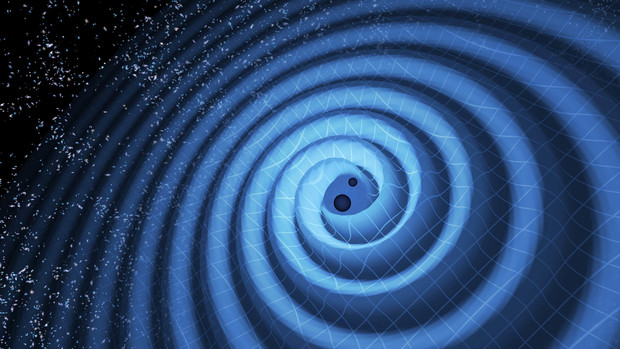
\includegraphics[width=\paperwidth,height=\paperheight]{Figures/GW-2.jpeg}}}

\begin{frame}[plain]
\titlepage

\begin{columns}
  \column{0.35\textwidth}
  \begin{figure}
    \centering
    \vspace{1.5mm}
    
\includegraphics[width=0.75\linewidth]{Figures/utrecht-university.png}
  \end{figure}
  \column{0.35\textwidth}
  \begin{figure}
    \centering
    
\includegraphics[width=0.75\linewidth]{Figures/Nikhef_logo-transparent.png}
  \end{figure}
\end{columns}

\end{frame}
}

% %The next statement creates the title page.
% \frame[plain]{\titlepage



% }


%---------------------------------------------------------
%This block of code is for the table of contents after
%the title page
% \begin{frame}[plain, noframenumbering]
% \frametitle{Table of Contents}
% \tableofcontents
% \end{frame}
%---------------------------------------------------------


\section{Introduction}

\begin{frame}{GW230529}

  \begin{figure}
    \centering
    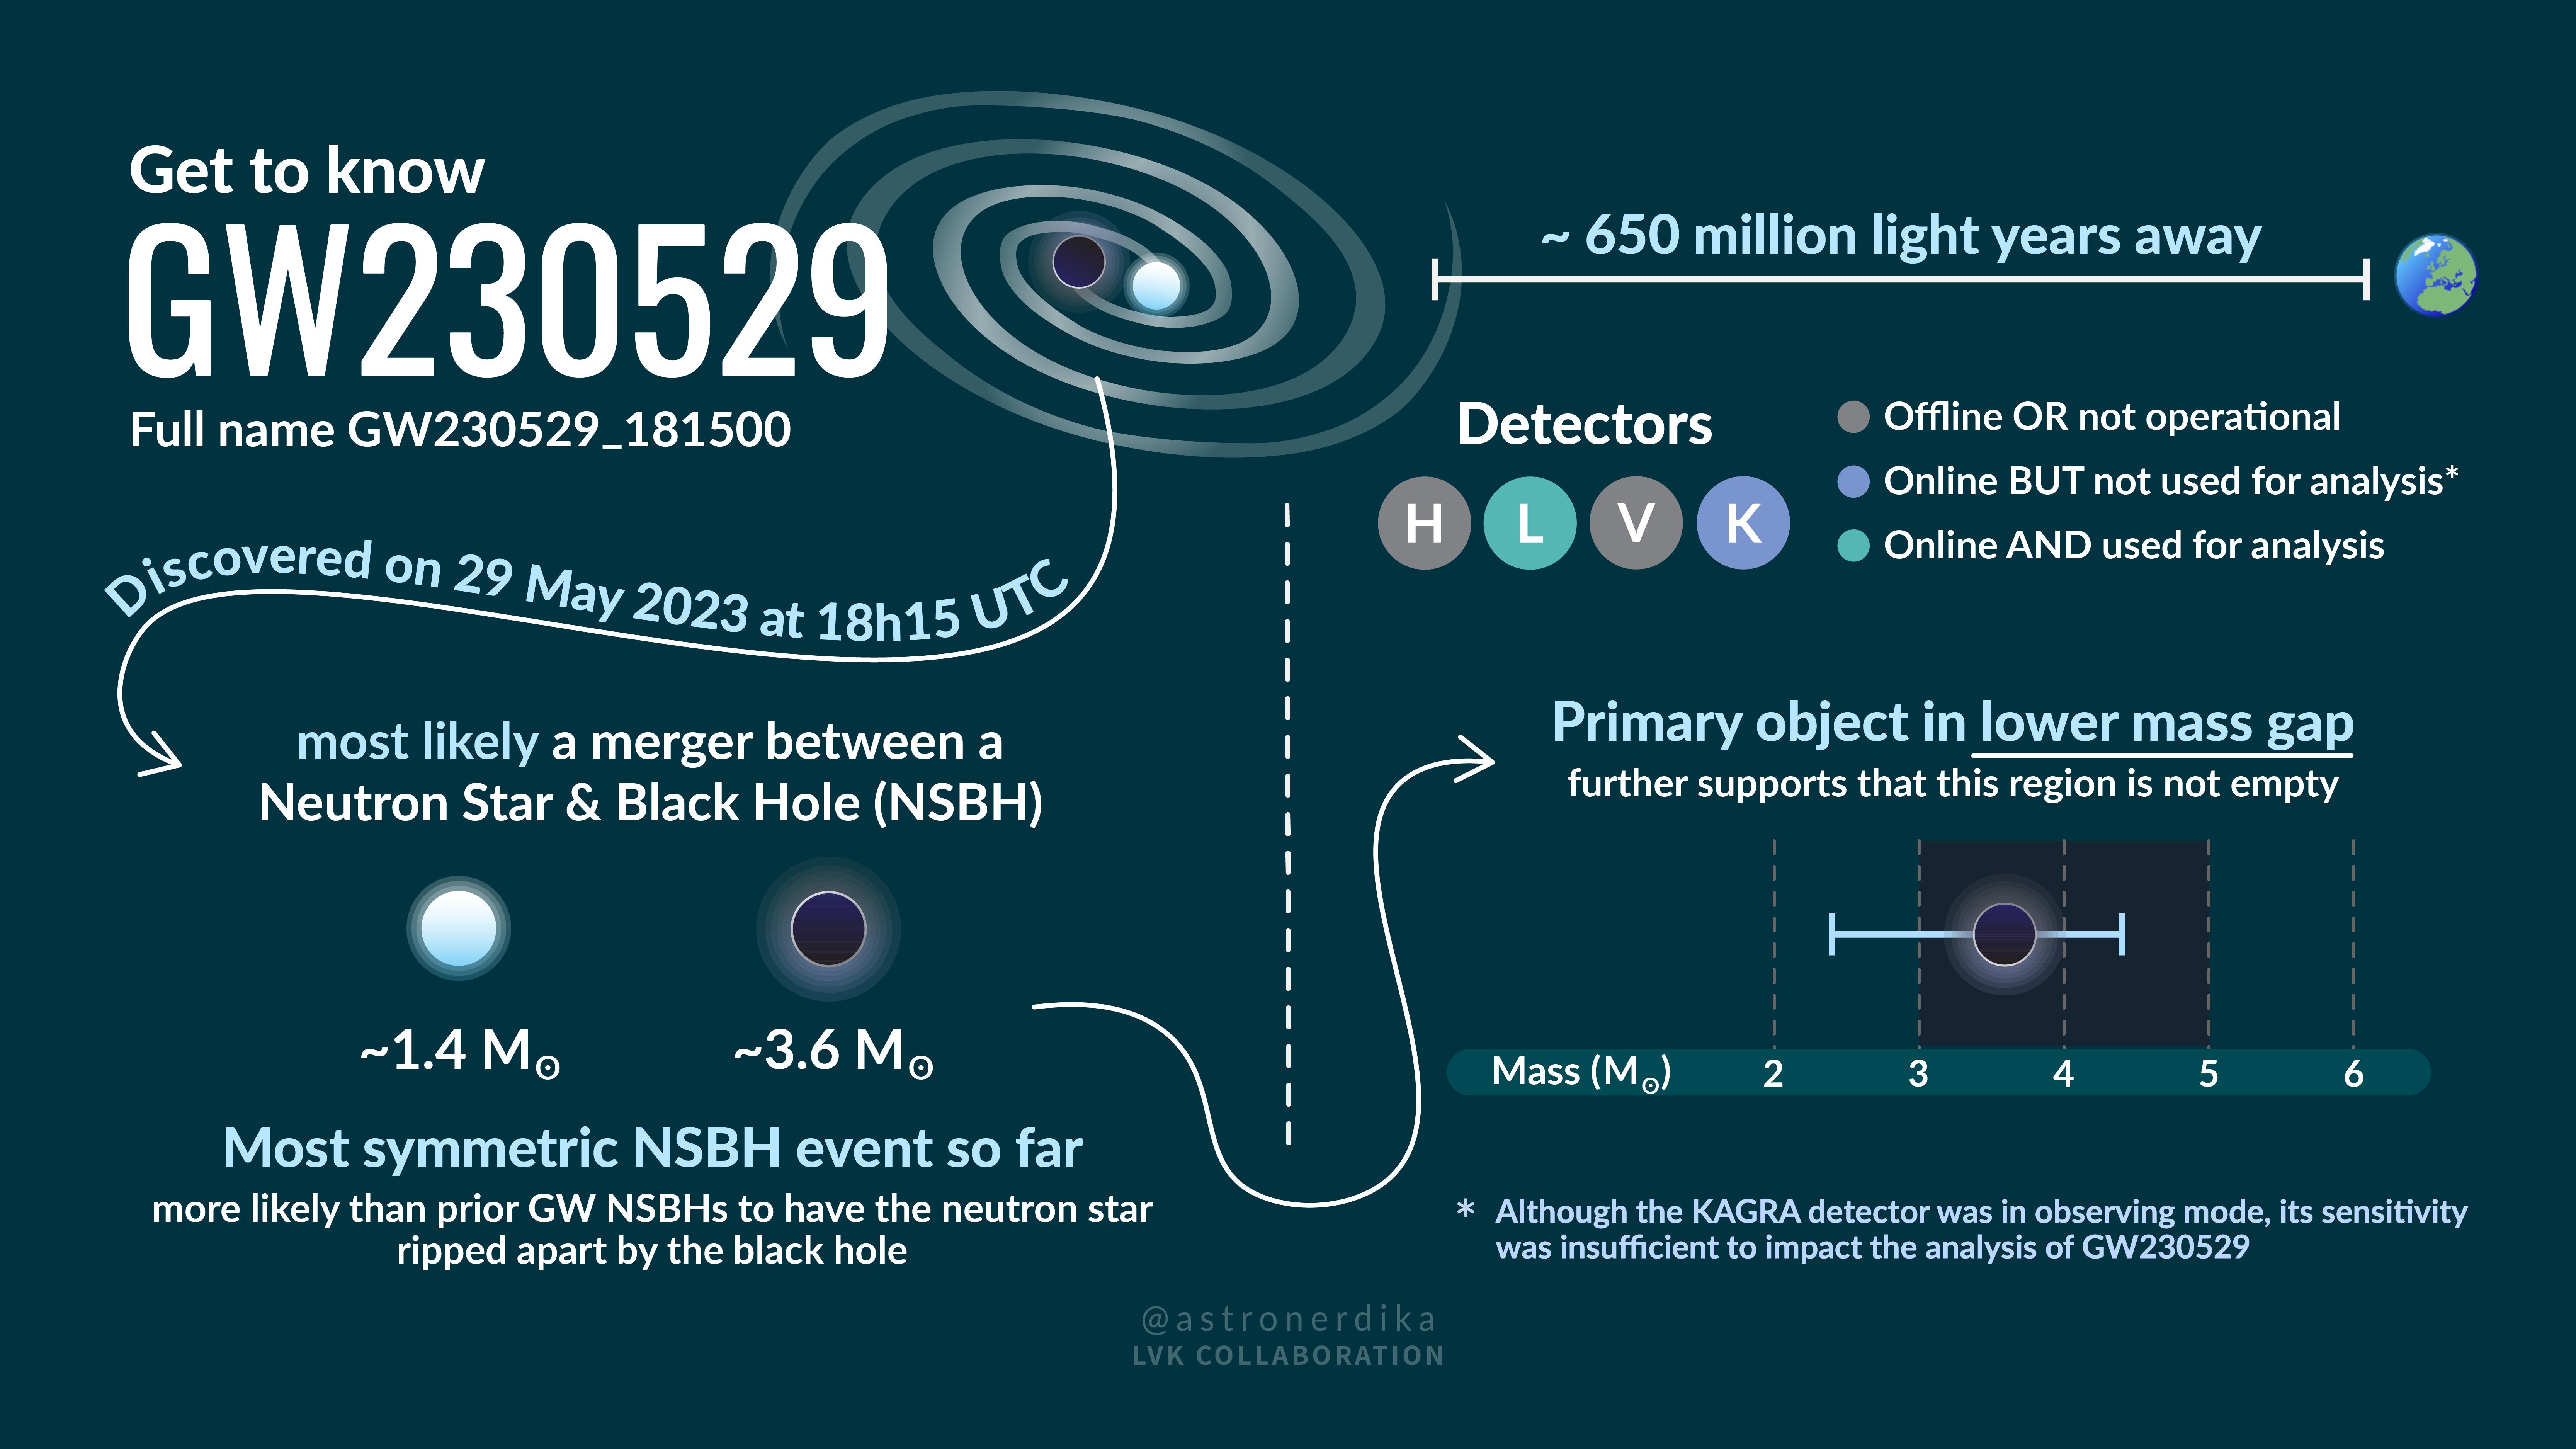
\includegraphics[width=1\linewidth]{Figures/GetToKnowGW230529_English.png}
  \end{figure}

  \scriptsize Credit: Shanika Galaudage \normalsize
\end{frame}

\section{Identifying GW230529's primary}

\begin{frame}{Identifying GW230529's primary}

  \def\x{3mm}
  \def\y{5mm}
  \def\z{1mm}

  What information can we get from GW230529?

  \vspace{\z}

  \begin{itemize}
    \item Tidal information? \red{uninformative}

    \vspace{\x}

    \item Electromagnetic counterpart? \red{not observed}

    \vspace{\x}

    \item $\rm{SNR} \approx 11$: \red{hard}

    \vspace{\x}

    \item Masses? \green{Well-measured!}
  \end{itemize}

  \vspace{\y}

  \pause

  Neutron stars have a maximal mass $M_{\rm{max}}$, which depends on the (unknown) equation of state and spin of the neutron star.

  \vspace{\x}

  \begin{tcolorbox}[colback=blue!10, boxrule=0pt]
    \textbf{Approach:} compare the mass distribution with expected upper bound
  \end{tcolorbox}
  
\end{frame}

\begin{frame}{Equation of state}

  \def\x{3mm}
  \def\y{3mm}

  \begin{itemize}

    \item Microscopically: nuclear interactions, $P(\epsilon, \rho)$,\dots
    
    \vspace{\x}
    
    \item Macroscopically: $M(R)$ $\rightarrow$ $\red{M_{\rm{TOV}}}$: maximum mass non-spinning neutron star
    
    \vspace{\x}
    
    \item Stars with spin $\chi$: $\red{M_{\rm{max}}}(\rm{EOS}, \chi) \lesssim 1.3 \ M_{\rm{TOV}}$. 
  \end{itemize}

  \vspace{\y}

  \only<1>{
  \begin{figure}
    \centering
    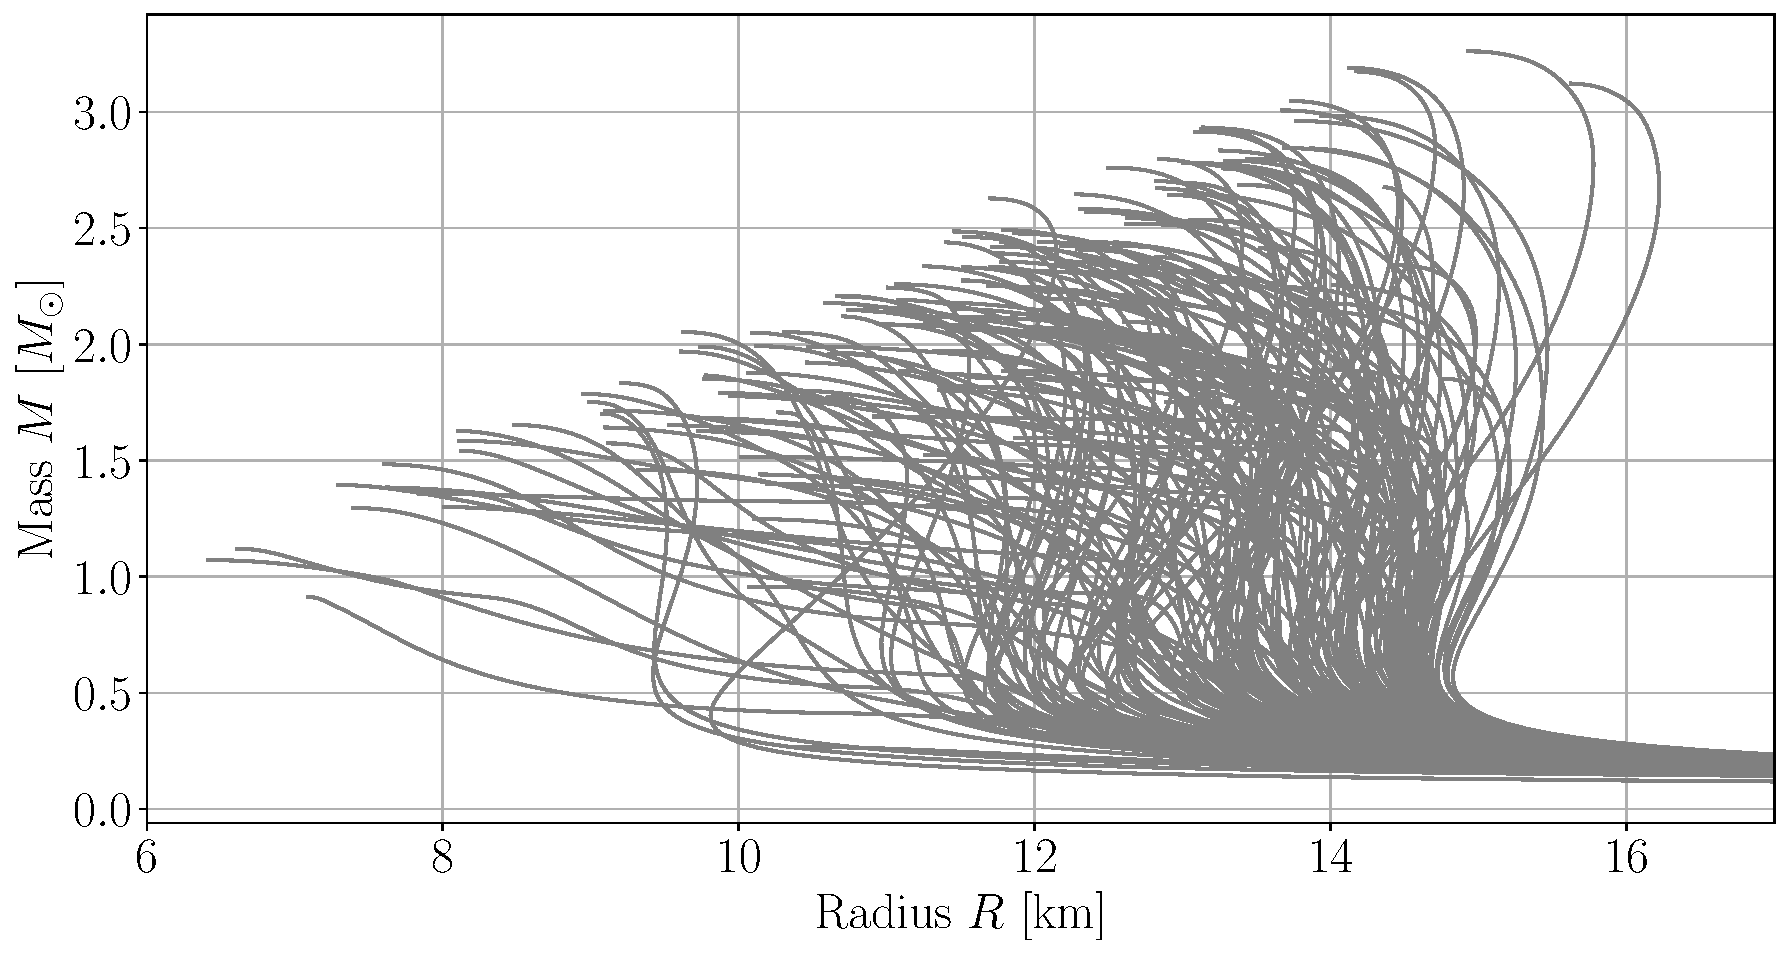
\includegraphics[width=0.75\linewidth]{Figures/mrl_samples.pdf}
  \end{figure}
  }

  % \only<2>{
  % \begin{figure}
  %   \centering
  %   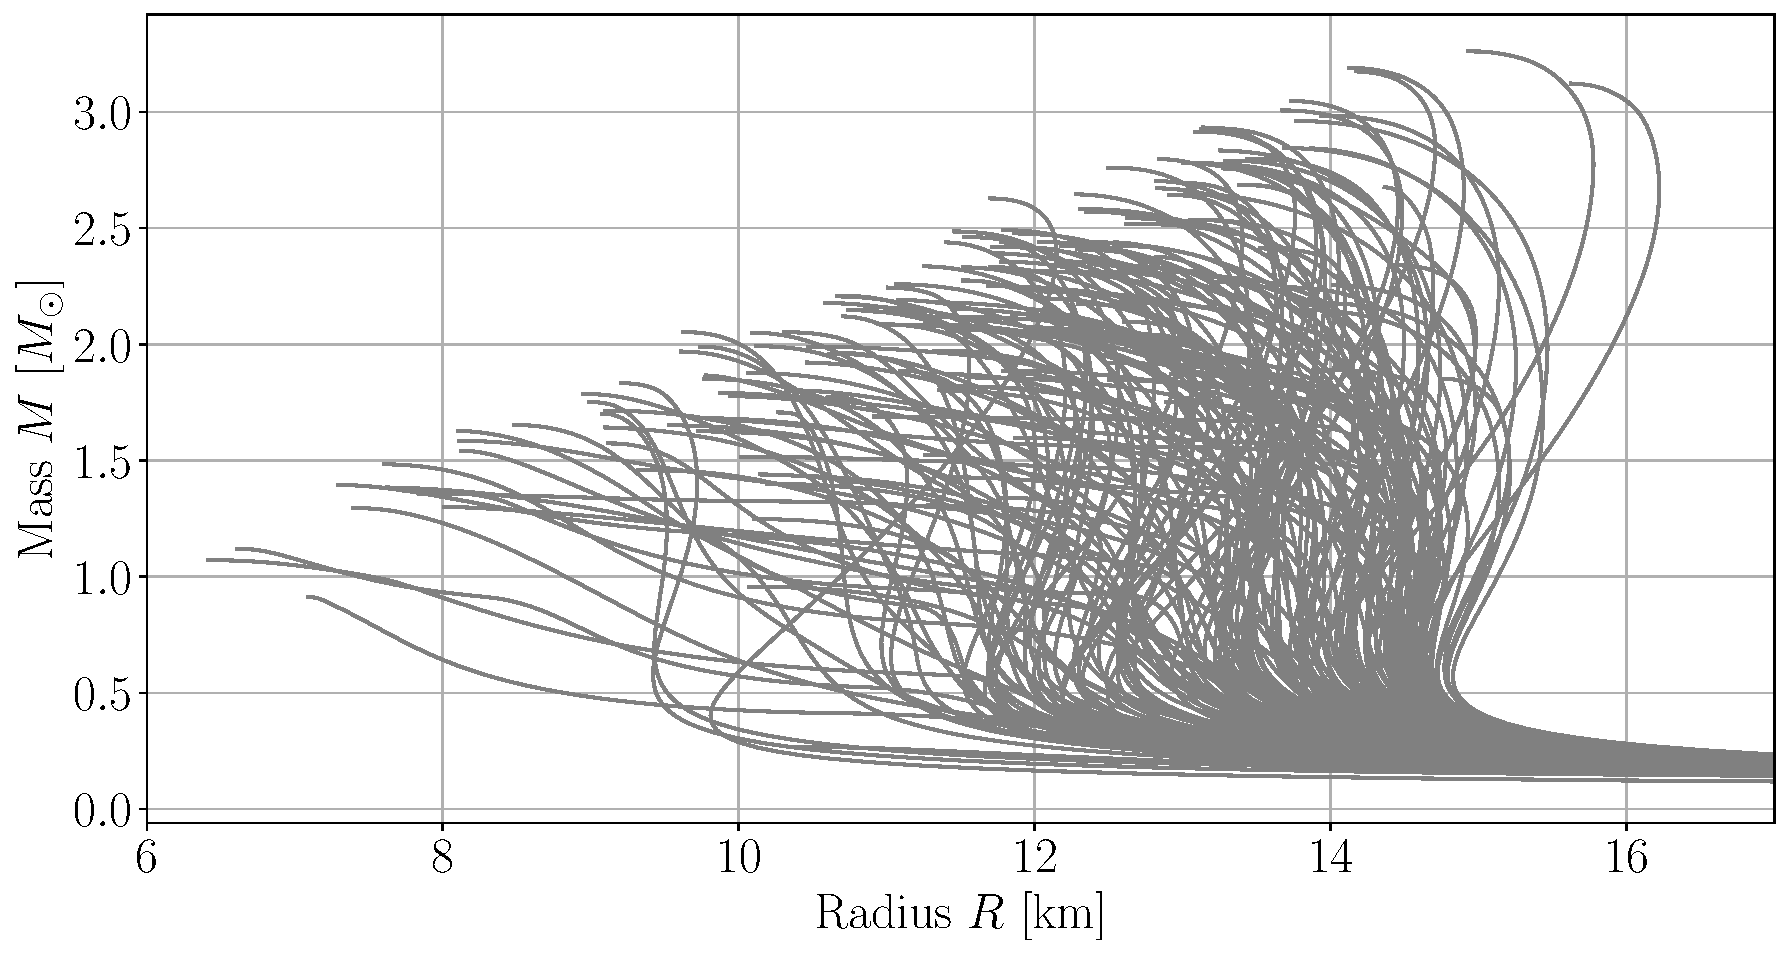
\includegraphics[width=0.75\linewidth]{Figures/mrl_samples.pdf}
  % \end{figure}
  % }
    
\end{frame}
\begin{frame}{Current equation of state constraints: \textsc{NMMA}}

\def\x{2mm}
\def\y{2mm}
\def\z{-2mm}

\vspace{\z}

\begin{columns}
  \column{0.9\textwidth}

  \textsc{NMMA} compiled a set of constraints on the equation of state:
  \footnotesize
  \begin{itemize}

    \item Nuclear theory and experiments
    \item Radio observations pulsars, NICER, bursters, X-ray binaries
    \item GW170817, EM counterparts, postmerger remnant

  \end{itemize}
  \normalsize
  \onslide<2->{
  Result: \blue{$M_{\rm{TOV}}$ posterior}
  }

  \column{0.1\textwidth}

  \begin{figure}[t]
    \centering
    
\includegraphics[width=\linewidth]{Figures/NMMA logo.jpg}
  \end{figure}
  
\end{columns}

\vspace{\x}
\onslide<2->{
\begin{figure}
  \centering
  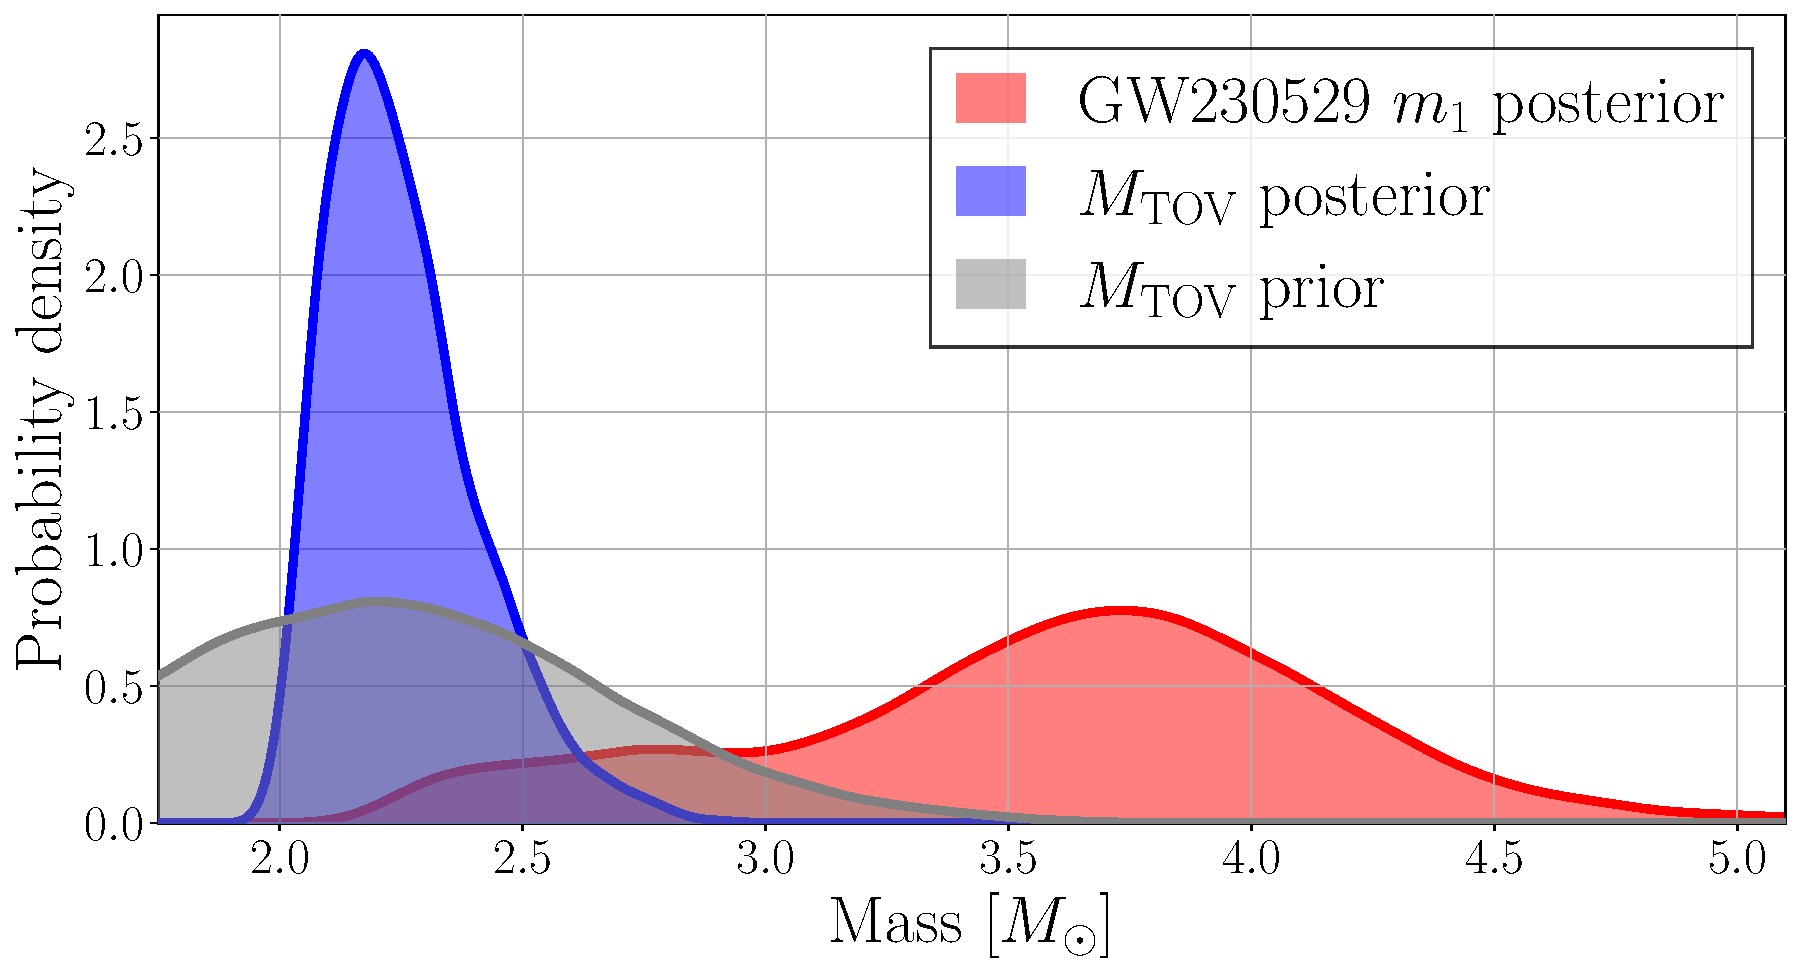
\includegraphics[width=0.7\linewidth]{Figures/mtov_gw230529_set_L1.pdf}
\end{figure}
}

\end{frame}

\begin{frame}{Identifying GW230529's primary: results}

  \def\heightlvk{2.25cm}
  \def\heightnmma{4.5cm}

  \def\x{2mm}
  \def\mycolwidth{4cm}
  \def\mycolwidthh{2cm}

  $P(NS)$: probability of primary being a neutron star

  \vspace{\x}

  \hrule

  \begin{minipage}[t][\heightlvk]{\textwidth}
    \begin{columns}
      \column{0.15\textwidth}

      \begin{figure}[t]
        \centering
        
\includegraphics[width=\linewidth]{Figures/LVK Logo.jpeg}
      \end{figure}
  
      \column{0.85\textwidth}

      \begin{table}
        \centering
        \begin{tabular}{| p{\mycolwidth} | p{\mycolwidthh} |}
          \hline
          \textbf{Posterior set} & $\mathbf{P(NS)}$ \\
          \hline
          default & $(2.9 \pm 0.4)\%$ \\
          population-informed & $(8.8 \pm 2.8)\%$ \\
          \hline
        \end{tabular}
      \end{table}

    \end{columns}
    \end{minipage}

    \hrule

    \vspace{1mm}

    \pause

    \vspace{1mm}

    \begin{minipage}[t][\heightnmma]{\textwidth}
      \begin{columns}
        \column{0.15\textwidth}
  
        \begin{figure}[t]
          \centering
          
\includegraphics[width=\linewidth]{Figures/NMMA logo.jpg}
        \end{figure}
        \begin{center}
          \textsc{NMMA}

          \scriptsize{\red{\textbf{PRELIMINARY!}}}
        \end{center}
    
        \column{0.85\textwidth}
  
        Without spin information, \textit{i.e.}, $M_{\rm{max}} = M_{\rm{TOV}}$:

        \begin{table}
          \centering
          \begin{tabular}{| p{\mycolwidth} | p{\mycolwidthh} |}
            % \hline
            % \textbf{Posterior set} & $\mathbf{P(NS)}$ \\
            \hline
            default & $\sim \phantom{0}1.63\%$ \\
            population-informed & $\sim \phantom{0}8.26\%$ \\
            \hline
          \end{tabular}
        \end{table}

        With spin information, \textit{i.e.}, $M_{\rm{max}} = M_{\rm{max}}(\rm{EOS}, \chi)$:

        \vspace{2mm}

        \begin{table}
          \centering
          \begin{tabular}{| p{\mycolwidth} | p{\mycolwidthh} |}
            % \hline
            % Posterior set & $P(NS)$ \\
            \hline
            default & $\sim \phantom{0}3.96 \%$ \\
            population-informed & $\sim 17.96 \%$ \\
            \hline
          \end{tabular}
        \end{table}
      \end{columns}
      \end{minipage}

      \hrule


  
\end{frame}

\section{Conclusion}

\begin{frame}{Conclusion}

  \def\x{7mm}

  \begin{itemize}
    \item GW230529: GW event with a component in the lower mass gap

    \vspace{\x}

    \item Hard to identify the primary: no electromagnetic counterpart, low $\rm{SNR}$,\dots

    \vspace{\x}

    \item Can use observational constraints on maximum mass of neutron stars

    \vspace{\x}

    \item \textsc{NMMA}: Extensive set of constraints on $M_{\rm{max}}$

    \vspace{\x}

    \item Primary object is a black hole (probability $82.04 \%$)
  \end{itemize}
  
\end{frame}

% \begin{frame}{References}

% % \nocite{*}
% \printbibliography
    
% \end{frame}

% ======== APPENDIX  ==========

\appendix

\begin{frame}[plain, noframenumbering]
\vfill
\centering
\textbf{APPENDIX}
\vfill
\end{frame}

\begin{frame}{$P(NS)$ definition}
  \begin{align*}\label{eq: probability of NS}
    \begin{split}
        P(\text{NS}) &= \sum_{\text{EOS}} P(\text{EOS}|d) \int_{0}^{\mtov(\text{EOS})} dm\ P(m|O) \\
                     &= \int d\mtov \int_{0}^{\mtov} dm\ P(\mtov|d) P(m|O)\\
                     &= \int_0^{\infty}\ d\Delta m \int_{-\infty}^{\infty} dm\ P(m+\Delta m|d) P(m|O).
    \end{split}
    \end{align*}
\end{frame}

\begin{frame}{Equation of state constraint sets}

  \small
\begin{table}[t]
  \renewcommand{\arraystretch}{1.1}
  \caption{Overview on the constraints contained within the three different constraint sets.}
  \label{tab:sets}
  \begin{tabular}{ l l p{7cm}}
  \toprule
  \toprule
  Set & Label & Description \\
  \midrule
  High confidence & 1 & Chiral EFT, pQCD, heavy radio pulsars, NICER \mbox{J0740+6620}, NICER \mbox{J0030+0451}, (NICER \mbox{J0437-4715}), GW170817\\
  \midrule
  More vigorous & 2 & Set 1, Black Widow \mbox{J0952-0607}, heavy ion-collisions, qLMXBs, GW170817+KN+GRB afterglow, CREX, PREX-II, Burster \mbox{4U 1702-429}, Burster \mbox{J1808.8-3658}, GW170817 postmerger\\
  \midrule
  Aggressive & 3 & Same as set 2, but for the remnant of GW170817 a hypermassive neutron star above the Kepler limit is assumed \\
  \bottomrule
  \end{tabular}
\end{table} 
\normalsize

\end{frame}

\begin{frame}{Population informed posterior}

  \begin{figure}
    \centering
    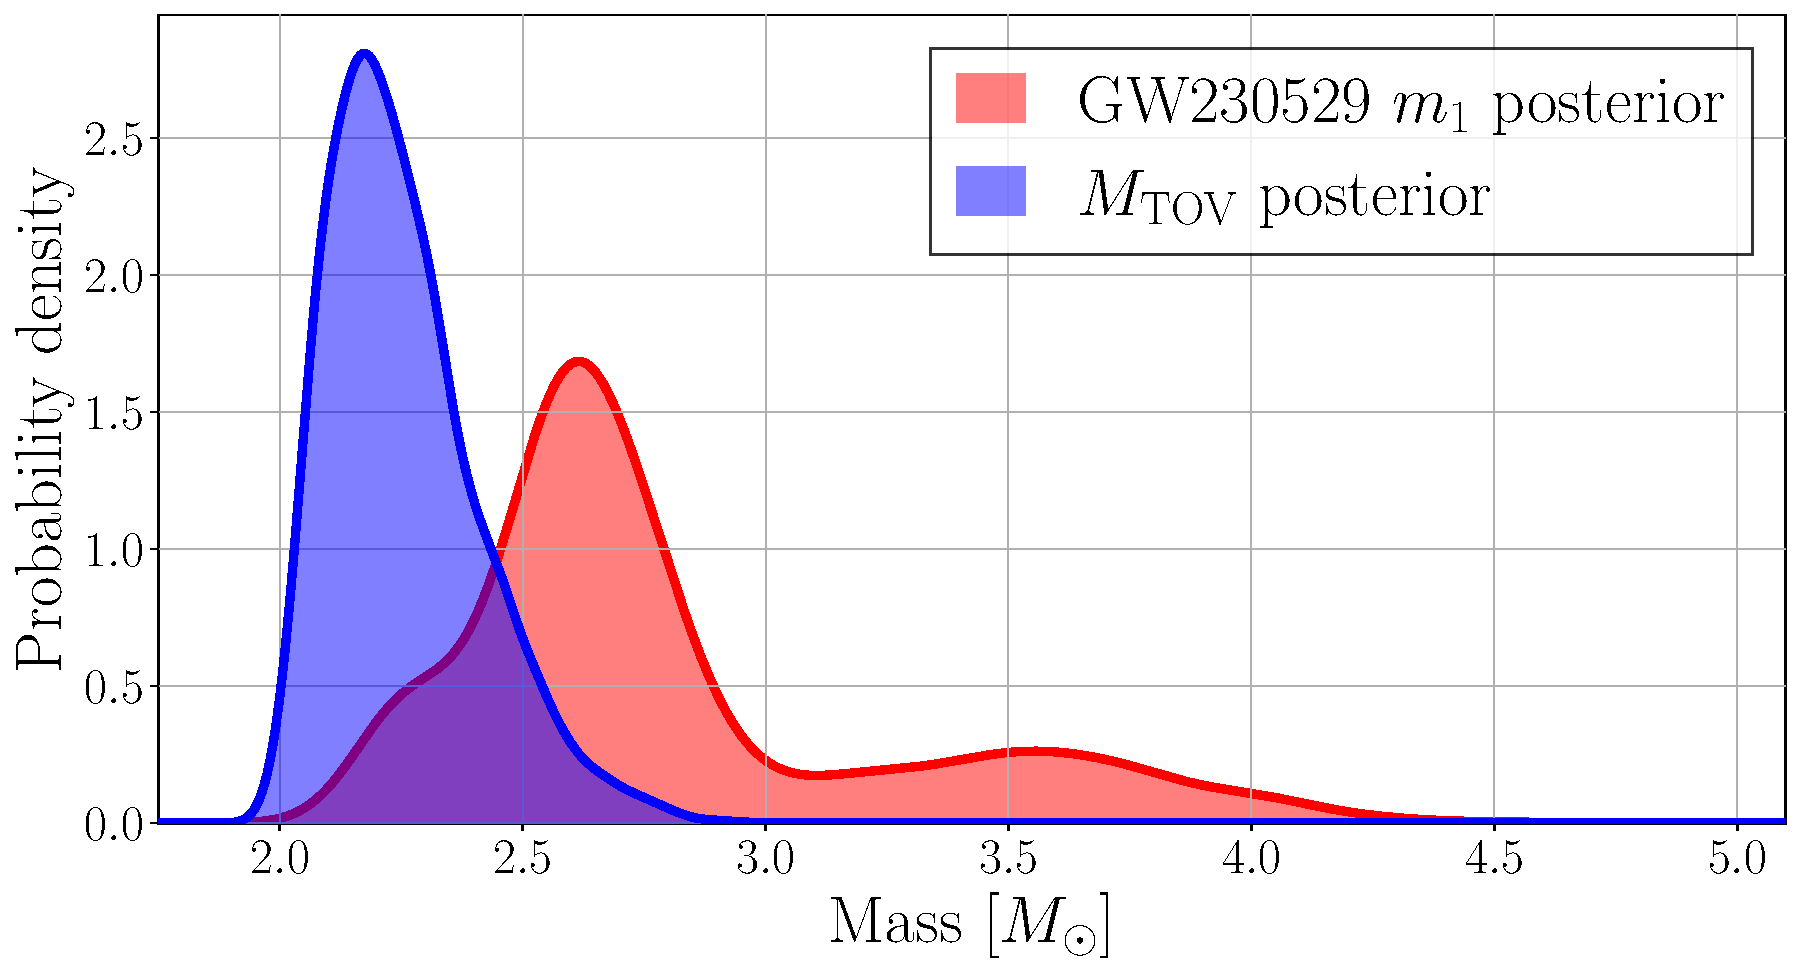
\includegraphics[width=0.9\linewidth]{Figures/mtov_gw230529_set_L1_pdb.pdf}
  \end{figure}    

\end{frame}

\begin{frame}{TOV mass posterior with set 3 (``Aggressive'')}

  \begin{figure}
    \centering
    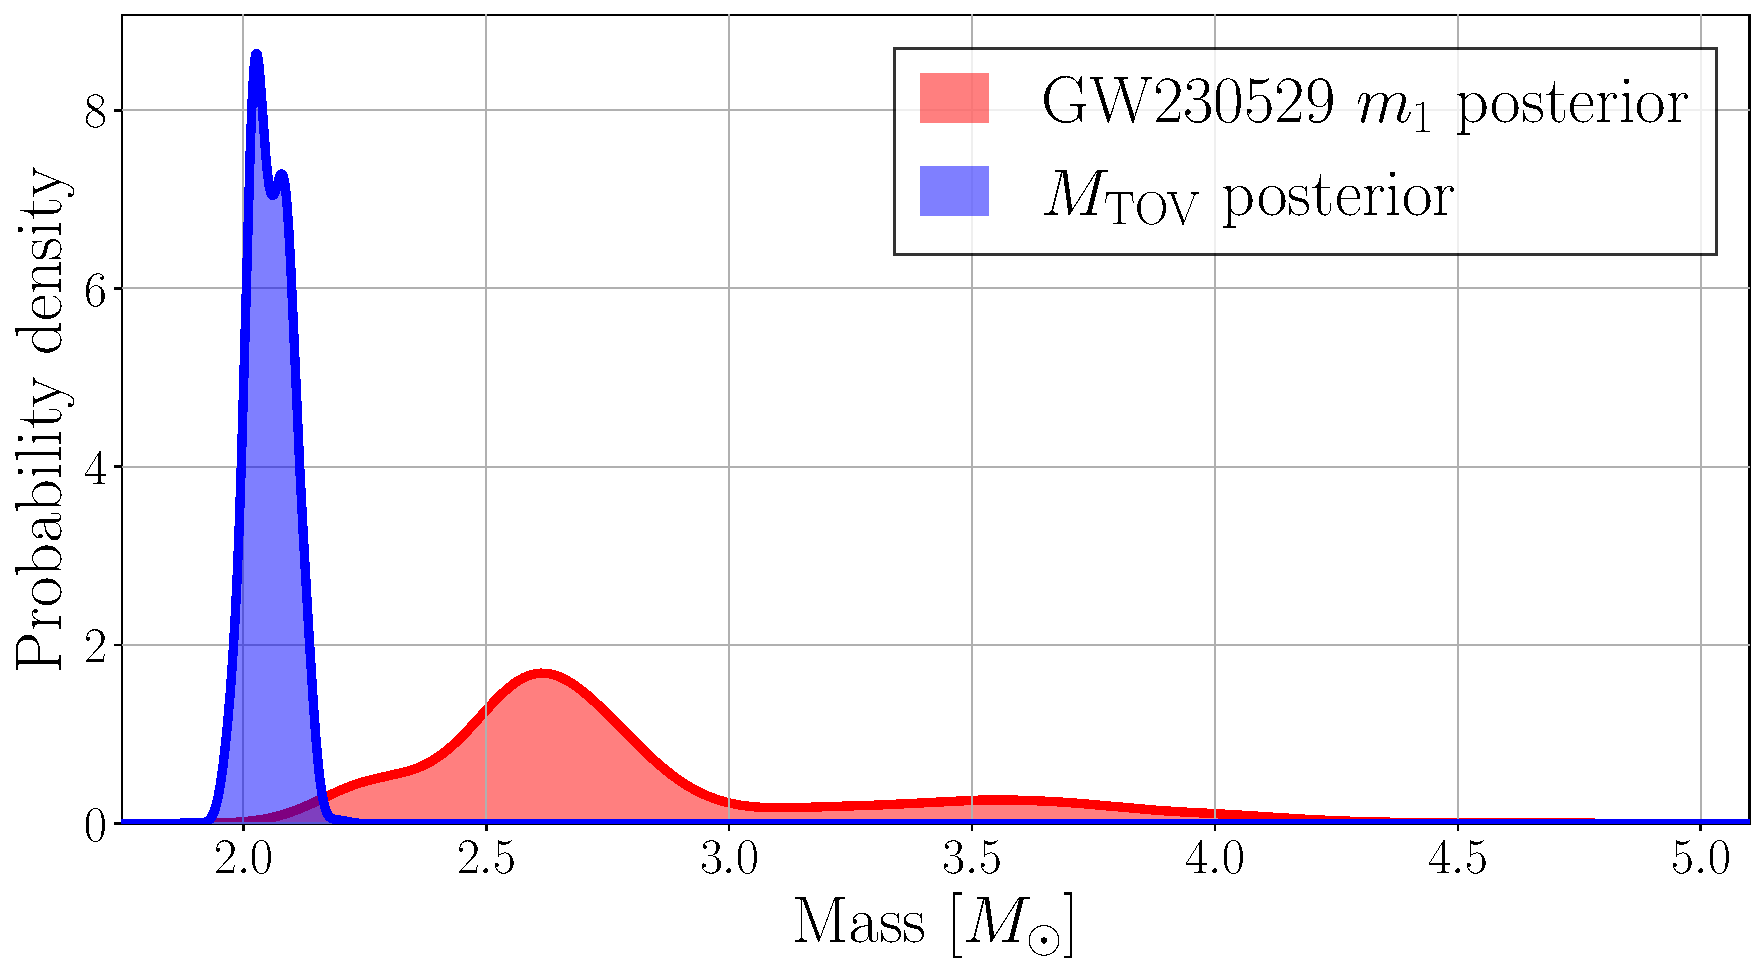
\includegraphics[width=0.75\linewidth]{Figures/mtov_gw230529_set_L3_pdb.pdf}
  \end{figure}

\end{frame}

\begin{frame}{All probabilities for GW230529 primary being a NS}

  \small
  \begin{table}
    \renewcommand{\arraystretch}{1.25}
    \centering
    % \caption{Probability that the primary component of GW230529 is a \ac{NS} when considering the posterior samples inferred when using the default priors (explained in the main text) and the priors informed by the \textsc{Power law + Dip + Break} (\textsc{PDB}) population model.}
    \label{tab: classification results GW230529}
    \begin{tabular*}{0.975\linewidth}{@{\extracolsep{\fill}} l c c | c c c}
\toprule\toprule
  & & spin & $1$ & $2$ & $3$ \\
\midrule
\multirow{4}{*}{GW230529} & \multirow{2}{*}{default} & $\cross$ & $\phantom{0}1.63\%$ & $\phantom{0}1.37\%$ & $\phantom{0}0.02\%$ \\ 
& & \checkmark & $\phantom{0}3.96\%$ & $\phantom{0}3.97\%$ & $\phantom{0}0.82\%$  \\ \cline{2-6}
& \multirow{2}{*}{\textsc{PDB}} & $\cross$ & $\phantom{0}8.26\%$ & $\phantom{0}6.98\%$ & $\phantom{0}0.38\%$ \\ 
& & \checkmark & $17.96\%$ & $17.83\%$ & $\phantom{0}1.79\%$ \\ 

\bottomrule
\end{tabular*}
\end{table}
\normalsize
\end{frame}


\end{document}